\subsection{D-Regler} % (fold)
\label{sub:D-Regler}
\begin{frame}
    \frametitle{D-Regler}
    \framesubtitle{}
    \begin{block}{Versuch}
        \begin{itemize}
            \item Untersuchung des D-Reglers
        \end{itemize}
    \end{block}
\end{frame}
\begin{frame}
    \frametitle{D-Regler}
    \framesubtitle{}
    \begin{columns}[c]
        \column{0.5\textwidth}
        \begin{block}{Beobachtung}
            \begin{itemize}
                \item T fällt in beiden Fällen stark ab
            \end{itemize}
        \end{block}
        \begin{block}{Erklärkung}
            \begin{itemize}
                \item 
                \begin{equation*}
                    D = t_d \frac{d (W-X)}{dt} = \frac{-X}{dt}
                \end{equation*}
                \item für $T>0$ ist $D < 0$
                \item D-Regler "weiß nichts" vom Sollwert
            \end{itemize}
        \end{block}
        \column{0.5\textwidth}
            \begin{figure}[H]
            \begin{center}
                    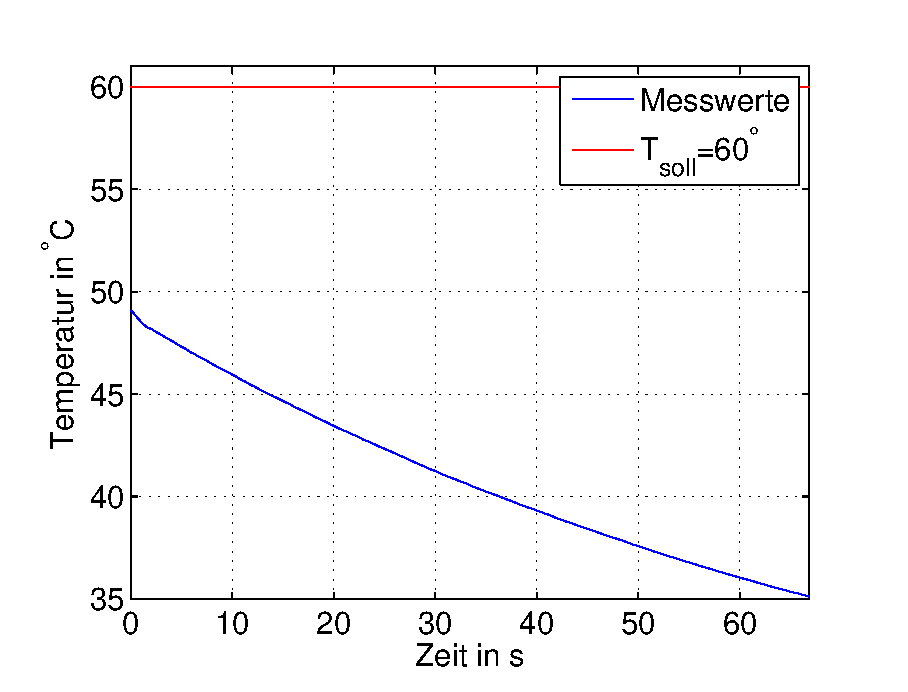
\includegraphics[scale=0.3]{./img/plots/2_e_td_1.eps}
            \end{center}
            \end{figure}
            \begin{figure}[H]
            \begin{center}
                    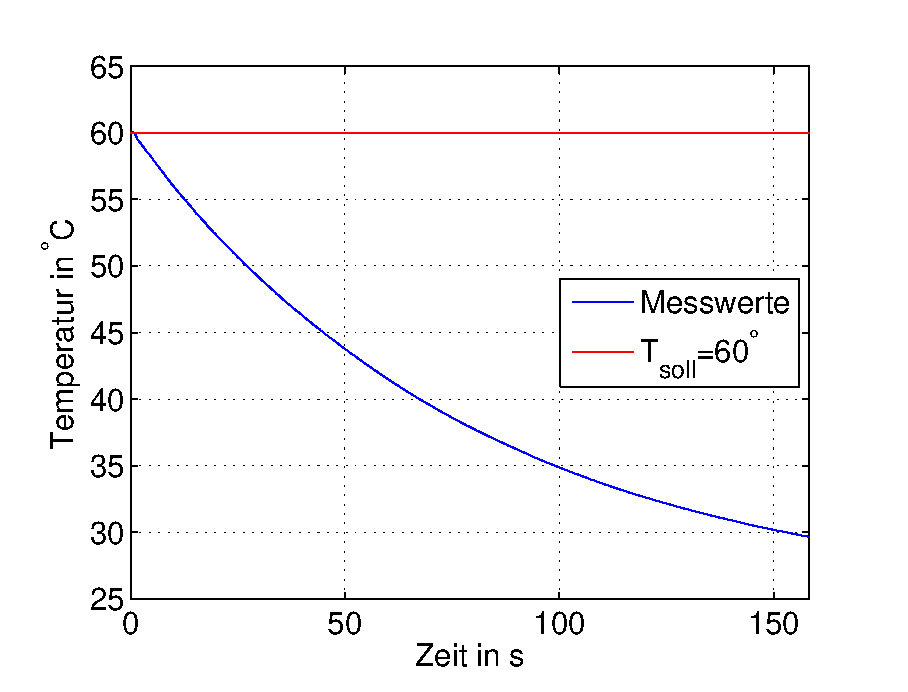
\includegraphics[scale=0.3]{./img/plots/2_e_td_1_2.eps}
            \end{center}
            \end{figure}
    \end{columns}
\end{frame}
% subsection D-Regler (end)
